\font\biggfnt=cmr10 scaled 1728
\font\rm=cmr9\rm\baselineskip11.5pt
\font\bf=cmbx9
\font\it=cmti9
\font\vv=cmcsc10 scaled 900
\font\rmsiete=cmr7
\font\itsiete=cmti10 scaled 700

\newdimen\altobull	\altobull=.8pt
\newbox\cajabull	\setbox\cajabull=\hbox{$\scriptscriptstyle\bullet$}
\newdimen\anchobull	\anchobull=\wd\cajabull	\advance\anchobull by .6pt

\def\eeb{\cr\noalign{\vskip\altobull}\reglao}
\def\eec{\cr\noalign{\vskip\altobull}}
\def\numazt#1#2{\hbox{\vtop to0pt{\vss\tabskip=0pt\offinterlineskip
  \halign{##\hfil\cr #2\cr\noalign{\vskip\altobull} #1\cr}}}}
\def\reglao{\hbox to 5\anchobull{\null\hfill}}
\def\regla{\hbox{\punto\punto\punto\punto\punto}}
\def\dregla{\hbox{\vbox{\tabskip=0pt\offinterlineskip
  \halign{##\hfil\cr\regla\cr\noalign{\vskip\altobull}\regla\cr}}}}
\def\punto{\rlap{$\scriptscriptstyle\bullet$}\hskip\anchobull}
\def\uno{\numazt{\punto\eeb\eeb}{\reglao\cr\reglao}}
\def\dos{\numazt{\punto\eec\punto\eeb}{\reglao\cr\reglao}}
\def\tres{\numazt{\punto\eec\punto\eec\punto}{\reglao\cr\reglao}}
\def\cuatro{\numazt{\punto\eec\punto\eec\punto\eec\punto}{\reglao}}
\def\cinco{\numazt{\eeb\eeb}{\reglao\cr\regla}}
\def\seis{\numazt{\punto\eeb\eeb}{\reglao\cr\regla}}
\def\siete{\numazt{\punto\eec\punto\eeb}{\reglao\cr\regla}}
\def\ocho{\numazt{\punto\eec\punto\eec\punto}{\reglao\cr\regla}}
\def\nueve{\numazt{\punto\eec\punto\eec\punto\eec\punto}{\regla}}
\def\diez{\numazt{\eeb\eeb}{\dregla}}
\def\once{\numazt{\punto\eeb\eeb}{\dregla}}
\def\doce{\numazt{\punto\eec\punto\eeb}{\dregla}}
\def\trece{\numazt{\punto\eec\punto\eec\punto}{\dregla}}

\def\glifo#1#2#3{\vbox to#2{\hsize#1
  \hrule height#2 depth0pt width0pt
  \noindent\special{pdf:image width #1 height #2 (#3.jpg)}}}

\def\'#1{\accent19\ifx#1i\i\else #1\fi}

\parskip0pt
\parindent12pt
\frenchspacing

\special{pdf:pagesize width 11truein height 8.5truein}

\noindent\hfill {\biggfnt Relaci\'on de los calendarios gregoriano y
azteca}\hfill\null

\vfill
\noindent Aunque la cuenta de los d\'ias y de los meses que formaban un a\~no
solar ten\'ia entre los nahuas menor importancia que el calendario de los
vaticinios ({\it Tonalpohualli\/}), presentamos el a\~no solar azteca por la
facilidad de adaptarlo al calendario gregoriano (que rige a la cultura
occidental en su mayor parte). El inter\'es principal que tiene este trabajo
es divulgar el arte prehisp\'anico en M\'exico, y no establecer o apoyar
alg\'un criterio cient\'ifico o t\'ecnico sobre c\'omo med\'ian el tiempo los
antiguos mexicanos.

El calendario solar azteca es un ciclo de 52 a\~nos que se divide en cuatro
trecenas de a\~nos, cada uno diferenciado de los otros mediante la
asignaci\'on c\'iclica de uno de los jerogl\'ificos {\it T\'ecpatl\/}
(pedernal), {\it Calli\/} (casa), {\it Tochtli\/} (conejo) o {\it \'Acatl\/}
(carrizo) y uno de los d\'igitos del 1 al~13 (representados con puntos).

Cada a\~no azteca o {\it X\'ihuitl\/} consta de 18 meses, de 20 d\'ias cada
uno, y un mes con s\'olo cinco d\'ias y seis horas ({\it Nemontemi\/})
llamados {\it Cempohuallis}. Un posible significado para cada uno de los
nombres de los meses es el siguiente ({\it v\'eanse\/} [Del Paso y Troncoso,
pp.~106 y ss.] y [Sahag\'un]):

\vskip1pc
\noindent\hfill\vbox{\halign{#\hfil\quad&#\hfil\quad&#\hfil\cr
\noalign{\hrule height1pt\vskip2pt}
{\bf mes}&{\bf numen}&{\bf significado posible}\cr
\noalign{\vskip2pt\hrule\vskip4pt}
{\it Atlacaualo}&{\it Tl\'aloc\/}&Lo que dejan las aguas.\cr
{\it Tlacaxipehualiztli}&{\it Xipe t\'otec\/}&Desollamiento de gentes.\cr
{\it Tozoztontli}&{\it Tl\'aloc\/}&Velaci\'on.\cr
{\it Hueytozoztli}&{\it Tl\'aloc\/}&Gran velaci\'on.\cr
{\it T\'oxcatl}&{\it Tezcatlipoca\/}&Sequ\'ia.\cr
{\it Itzacualiztli\/}&{\it Tl\'aloc}, {\it Quetzalc\'oatl\/} y {\it
X\'olotl\/}&Preparaci\'on del {\it itzalli\/} (frijol y ma\'iz).\cr
{\it Tecuilhuitontli}&{\it Quetzalc\'oatl}, {\it Cihuac\'oatl},&Fiesta de los
se\~nores.\cr
  &\kern5pt {\it Cinte\'otl\/} y {\it Ixtl\'iltzin\/}&\cr
{\it Hueytecu\'ilhuitl}&{\it Cinte\'otl\/} y {\it Xipe t\'otec\/}&Gran
fiesta de los se\~nores.\cr
{\it Tlaxochimaco}&{\it Cihuac\'oatl\/}&Fiesta de las flores.\cr
{\it Xocothuetzi}&{\it Xiuteuctli\/}&Maduraci\'on de los frutos.\cr
{\it Ochpaniztli}&{\it Toci}, {\it Xicomec\'oatl\/} y {\it
Atlat\'onan\/}&\'Epoca de la limpieza (cosecha).\cr
{\it Teotleco}&{\it Xochiquetzalli}, {\it Tezcatlipoca\/} y&Llegada de los
dioses.\cr
  &\kern6pt {\it Huitzilopochtli\/}&\cr
{\it Tepe\'ihuitl}&{\it Xochiquetzalli}, {\it Tl\'aloc\/} y {\it
Napatecutli\/}&Fiesta de los cerros.\cr
{\it Quecholli}&{\it Mixc\'oatl\/} y {\it Tezcatlipoca
tlamatcincatl\/}&Fiesta de las flechas.\cr
{\it Panquetzalistli}&{\it Huitzilopochtli\/}&Despliegue de banderas.\cr
{\it Atemoztli}&{\it Chalchiuitl\/}&Descenso de las aguas.\cr
{\it T\'ititl}&{\it Cihuac\'oatl\/}&Resurgimiento de la naturaleza.\cr
{\it Izcalli}&{\it Xiuteuctli\/}&Surgimiento de la naturaleza.\cr
{\it Nemontemi}&&D\'ias festivos.\cr
\noalign{\vskip4pt\hrule height1pt}}}\hfill\null
\vskip1pc

Los d\'ias aztecas se agrupan en trecenas que se relacionan uno a uno con 20
jerogl\'ificos en forma c\'iclica, excepto los cinco d\'ias y seis horas del
mes {\it Nemontemi}, que carecen tanto de numeral como de numen.

Los trece numerales se representan mediante un n\'umero correspondiente de
puntos, y los nombres que se les asignan son:

\vskip1pc
\noindent\hfill\vbox{\halign{#\hfil\ &#\hfil\quad&#\hfil\ &#\hfil\quad&
  #\hfil\ &#\hfil\quad&#\hfil\ &#\hfil\quad&#\hfil\ &#\hfil\cr
\noalign{\hrule height1pt\vskip12pt}
  \uno&Ce&\dos&Ome&\tres&Yei&\cuatro&Nahui&\cinco&Macuilli\cr\cr\cr
  \seis&Chicuace&\siete&Chicome&\ocho&Chicuei&\nueve&Chiconahui&
    \diez&Matlactli\cr\cr\cr
  \once&Matlactlionce&\doce&Matlactliomome&\trece&Matlactliomei&&&&\cr
\noalign{\vskip6pt\hrule height1pt}}}\hfill\null

\eject

Los nombres de los n\'umenes son:

\vskip1pc
\noindent\hfill\vbox{\rmsiete\halign{\hfil#\ &#\hfil\quad&\hfil#\ &
  #\hfil\quad&\hfil#\ &#\hfil\quad&\hfil#\ &#\hfil\cr
\noalign{\hrule height1pt\vskip2pt}
    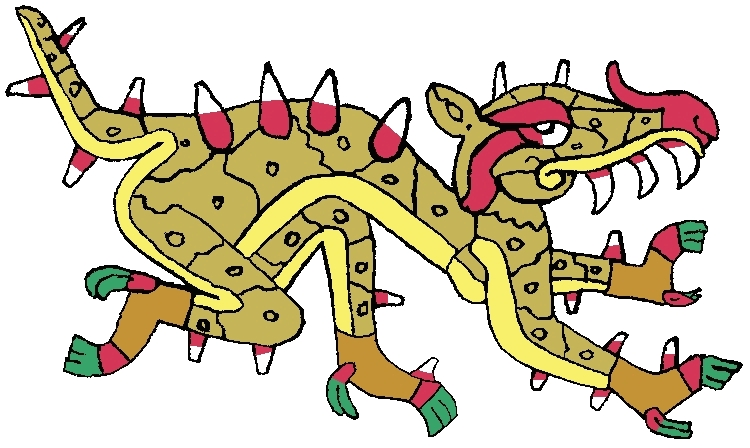
\includegraphics[width=62pt,height=36pt]{cipactli.jpg}&{\itsiete Cipactli\/} (caim\'an),&
    
\includegraphics[width=41pt,height=36pt]{ehecatl.jpg}&{\itsiete Eh\'ecatl\/} (viento),&
    
\includegraphics[width=25pt,height=36pt]{cali.jpg}&{\itsiete Calli\/} (casa),&
    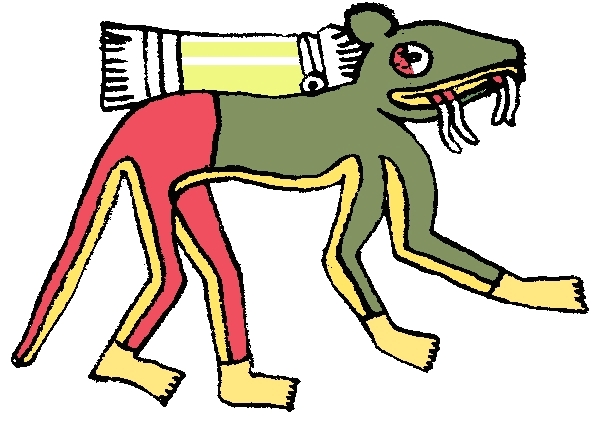
\includegraphics[width=50pt,height=35pt]{cuespali.jpg}&{\itsiete Cuetspallin\/} (lagartija),\cr
  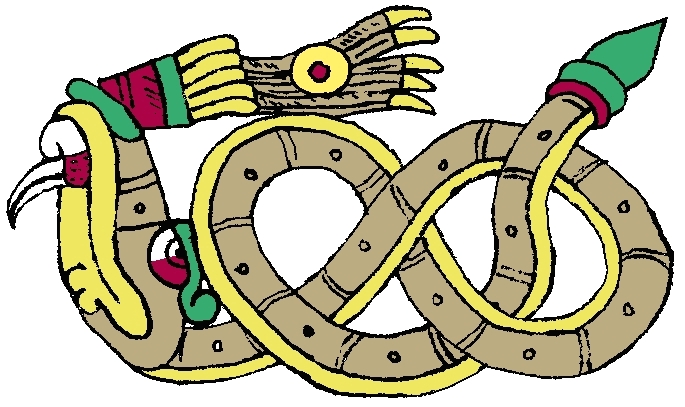
\includegraphics[width=58pt,height=34pt]{coatl.jpg}&{\itsiete C\'oatl\/} (serpiente),&
    
\includegraphics[width=23pt,height=36pt]{mikistli.jpg}&{\itsiete Miquistli\/} (muerte),&
    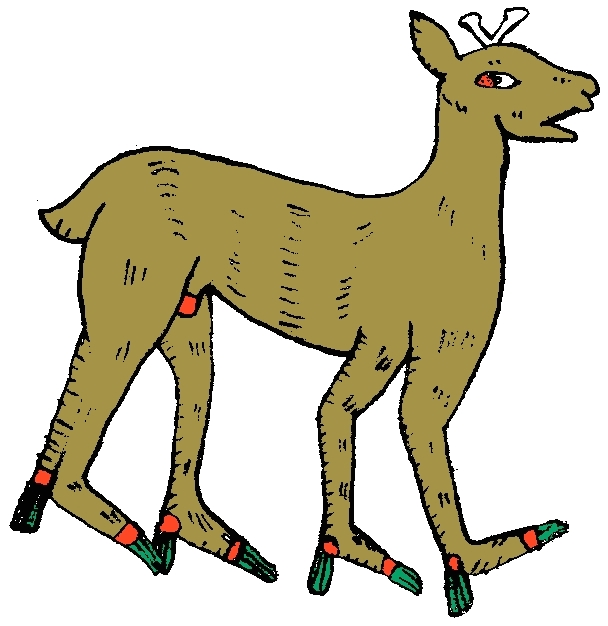
\includegraphics[width=35pt,height=36pt]{mazatl.jpg}&{\itsiete M\'azatl\/} (venado),&
    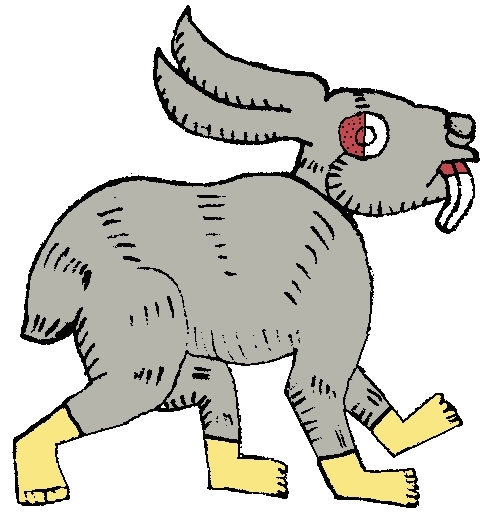
\includegraphics[width=34pt,height=36pt]{tochtli.jpg}&{\itsiete Tochtli\/} (conejo),\cr
  
\includegraphics[width=50pt,height=35pt]{atl.jpg}&{\itsiete Atl\/} (agua),&
    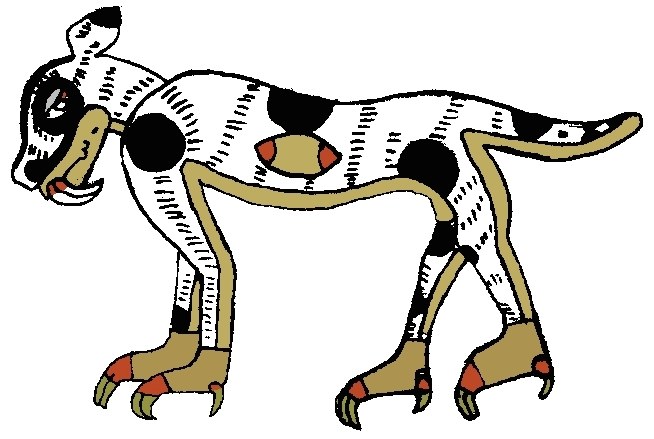
\includegraphics[width=53pt,height=36pt]{scuintli.jpg}&{\itsiete Itzcuintli\/} (perro),&
    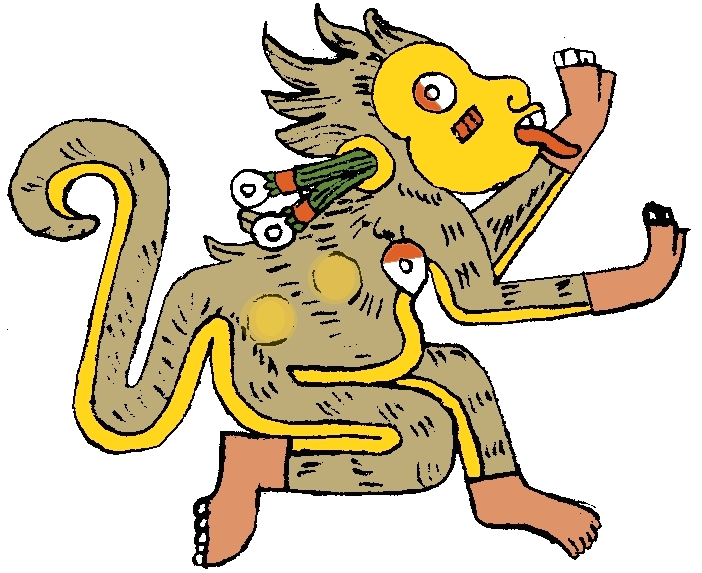
\includegraphics[width=42pt,height=35pt]{osomatli.jpg}&{\itsiete Osomatli\/} (mona),&
    
\includegraphics[width=47pt,height=35pt]{malinali.jpg}&{\itsiete Malinalli\/} (hierba),\cr
  
\includegraphics[width=28pt,height=36pt]{acatl.jpg}&{\itsiete \'Acatl\/} (carrizo),&
    
\includegraphics[width=24pt,height=36pt]{ocelotl.jpg}&{\itsiete Oc\'elotl\/} (ocelote),&
    
\includegraphics[width=53pt,height=34pt]{cuautli.jpg}&{\itsiete Cuauhtli\/} (\'aguila),&
    
\includegraphics[width=51pt,height=36pt]{coscacua.jpg}&{\itsiete Coscacuauhtli\/} (\'aguila real),\cr
  
\includegraphics[width=36pt,height=35pt]{olin.jpg}&{\itsiete Ollin\/} (movimiento),&
    
\includegraphics[width=21pt,height=36pt]{tecpatl.jpg}&{\itsiete T\'ecpatl\/} (pedernal),&
    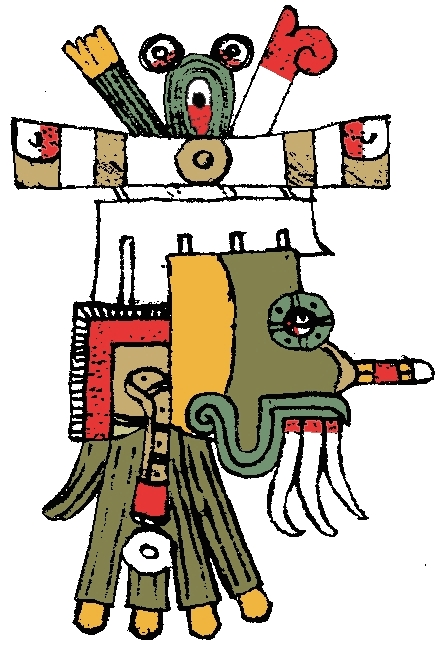
\includegraphics[width=25pt,height=36pt]{kiauitl.jpg}&{\itsiete Qui\'ahuitl\/} (lluvia) y&
    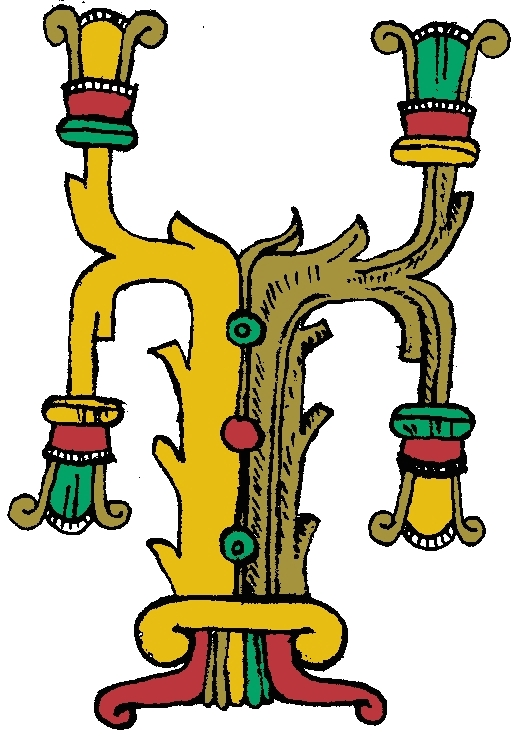
\includegraphics[width=25pt,height=36pt]{xochitl.jpg}&{\itsiete Xochitl\/} (flor).\cr
\noalign{\vskip6pt\hrule height1pt}}}\hfill\null
\vskip1pc

Supuesto que cada a\~no azteca tiene 365 d\'ias y 6 horas, \'estos se suceden
comenzando a diferente hora del d\'ia en un periodo de cuatro a\~nos. As\'i,
los a\~nos {\it Tochtli\/} comienzan al amanecer o {\it Iquiza Tonatiuh}, los
a\~nos {\it \'Acatl\/} al mediod\'ia o {\it Nepantla Tonatiuh}, los a\~nos
{\it T\'ecpatl\/} al anochecer u {\it Onaqui Tonatiuh} y, finalmente, los
a\~nos {\it Calli\/} a la media noche o {\it Yohualnepantla}.

El criterio de conciliaci\'on de fechas entre los calendarios azteca y
gregoriano parte de la fecha {\it Ce C\'oatl}, {\it Tlaxochimaco}, {\it Yei
Calli\/} (d\'ia uno serpiente, del mes en que se celebra la fiesta de las
flores, del a\~no tres casa), o 13 de agosto de 1521 (del calendario juliano),
en que los espa\~noles tomaron la ciudad de Tenochtitlan.

Los dibujos y los colores de los n\'umenes se hicieron tomando como base los
jerogl\'ificos que aparecen en el C\'odice Borgia, comentado por Seler y
editado por el {\vv fce} [Seler], sin deseo de copiar o igualar la calidad de
aqu\'ellos. Deseamos enfatizar que en este trabajo no se pretende establecer o
apoyar criterio alguno sobre c\'omo med\'ian el tiempo los aztecas.

El C\'odice Borgia pertenece al grupo de los calendarios religiosos augurales;
sin embargo, contiene dise\~nos muy hermosos y fue esa la raz\'on de que
\'estos se tomaran de all\'i ({\it cf.} [Nuttall]). La digitalizaci\'on se
realiz\'o con un {\it ScanJet Plus\/} de Hewlett Packard con resoluci\'on de
300 puntos por pulgada en una PC. La tipograf\'ia se hizo inicialmente con \TeX\
([Knuth]) y el archivo .PDF se generó con WinEdt 6 [Build: 20101215 (v.6.0);
For: Windows 7, Vista, XP, 2000]. Ahora (2024) lo adaptamos a \LaTeX\ y el
archivo .PDF se generá usando TeXworks, versión 0.6.8 (MiKTeX 23.10).

Existe además una versi\'on del calendario que escribmos en formato HTML
([Lemay] y [Powell]), en el sitio
\href{http://www.uaq.mx/ingenieria/publicaciones/calendarios/calazt.html}{\tt
http://www.uaq.mx/ingenieria/publicaciones/calendarios/calazt.html}, para la
Universidad Aut\'onoma de Quer\'etaro, Qro., M\'exico. También programamos una
versión (1.3) en Java (2021) que nos permite incluir foto con referencia en
los días (como cumpleaños) y una {\tt app} con {\it Android Studio\/} que
estamos depurando y que probablemente reescribamos en Kotlin.

Las fechas de las fases de la Luna fueron calculadas con un programa escrito
en~C ([Kernighan {\it et al.}], [Lattice] y [Press {\it et al.}]).

\noindent\hfill {\vv Miguel Navarro Saad}

\def\.{\noindent\hangindent1pc\hangafter1\ignorespaces}

\vskip2pc
\.Del Paso y Troncoso, Francisco, {\it Descripci\'on, historia y exposici\'on
del C\'odice Borb\'onico}, edici\'on facsimilar, Siglo Veintiuno, M\'exico,
1985.

\.Hewlett-Packard, {\it Guide to the HP ScanJet Plus Scanner}, HP~9195A/AB,
1990.

\.Kernighan, Brian W., y Dennis M. Richtie, {\it The C Programming Language},
Second Edition, Prentice Hall Software Series, New Jersey, 1988.

\.Knuth, Donald E., {\it The \TeX book}, Addison-Wesley Publishing Company,
American Mathematical Society, {\vv eua}, 1984.

\.Lattice, Inc., {\it Lattice C Compiler for 8086/8088 Series Microprocessor},
Version~2.15, Glen Ellyn, IL., 1985.

\.Lemay, Laura, {\it Aprendiendo HTML~4 para WEB en una semana}, tercera
edici\'on, SAMS, Prentice Hall, M\'exico, 1998.

\.Nuttall, Zelia (Ed.), {\it The Codex Nuttall. A Picture Manuscript from
Ancient Mexico}, Dover Publications, Inc., New York, 1975.

\.Powell, Thomas A., {\it HTML: Manual de referencia}, Osborne McGraw-Hill,
Espa\~na, 1998.

\.Press, William H., Brian P. Flannery, Saul A. Teukolsky y William T.
Vetterling, {\it Numerical Recipes in~C. The Art of Scientific Computing},
Cambridge University Press, {\vv eua}, 1988.

\.Sahag\'un, Bernardino de, FR., {\it Historia general de las cosas de Nueva
Espa\~na}, novena edici\'on, Editorial Porr\'ua, M\'exico, 1997.

\.Seler, Eduard, {\it Comentarios al C\'odice Borgia}, Fondo de Cultura
Econ\'omica, M\'exico, 1980.
